% ═══════════════════════════════════════════════════════════════════════════════
% CHAPTER — PROPOSED SOLUTION
% End-of-Study Report — MES-X Dependency Traceability System
% ═══════════════════════════════════════════════════════════════════════════════

\chapter{Proposed Solution}
\label{chap:proposed-solution}

% ─────────────────────────────────────────────────────────────────────────────
\section{Introduction}
\label{sec:solution-intro}

The previous chapter showed that Azure DevOps stores the necessary traceability
data, but does not present it in a form that is easy to analyze end to end.
Teams therefore have to move manually between work items, pull requests,
commits, branches, and tags to reconstruct the dependency chain of a feature.
That approach is workable on a small scale, but it becomes costly and unreliable
in a large microservices environment.

The proposed solution addresses this gap through a \textbf{centralized
dependency traceability system} designed for Azure DevOps-based workflows.
Rather than replacing the existing platform, it adds an analytical layer on top
of it: the system retrieves data from Azure DevOps APIs, rebuilds dependency
graphs, enriches the raw artifacts with additional context, and exposes the
result through a dedicated interface.

The system is built around three guiding ambitions:

\begin{itemize}
  \item \textbf{Completeness}: Every artifact in the dependency chain — from
  epics and features down to individual commits and Git tags — must be
  reachable and traceable within a single analysis session.

  \item \textbf{Consistency}: All data must be normalized before processing so
  that results are stable and predictable regardless of the structural
  variations present in Azure DevOps API responses.

  \item \textbf{Actionability}: The final output must not be a raw data dump.
  It must be organized into structured, decision-ready views that directly
  support release readiness assessment, impact analysis, and dependency
  validation.
\end{itemize}

The following sections present the global architecture of the solution, the
design principles that govern its construction, the four core components that
form the traceability pipeline, the end-to-end data flow connecting them, and
the concrete advantages the system delivers over the current state of practice.


% ─────────────────────────────────────────────────────────────────────────────
\section{Global System Architecture}
\label{sec:global-architecture}

The system adopts a \textbf{three-layer architecture} that cleanly separates
the concerns of user interaction, business orchestration, and external data
access. This separation is not merely a structural convention: it is a
deliberate design decision that ensures each layer can be developed, tested,
and evolved independently without creating cascading changes across the system.

\begin{figure}[htbp]
  \centering
  
\includegraphics[width=\linewidth]{img/archi/general_archi.png}
  \caption{Global three-layer architecture of the proposed solution.}
  \label{fig:global-architecture}
\end{figure}

\subsection{Presentation Layer — Trace UI}
\label{subsec:presentation-layer}

The Presentation Layer is the entry point for end users. It is implemented as a
dedicated web interface — referred to throughout this document as the
\emph{Trace UI} — that allows users to initiate dependency analysis sessions,
monitor their progress in real time, and explore the resulting dependency graphs
and decision outputs.

The Trace UI is not a passive display surface. It actively participates in the
orchestration of the analysis by:

\begin{itemize}
  \item accepting user-defined analysis parameters (work item identifiers,
  project context, analysis mode);
  \item managing the lifecycle of asynchronous and streamed backend interactions;
  \item assembling and normalizing backend responses into a coherent view state;
  \item presenting structured, layered results across multiple specialized views.
\end{itemize}

The interface supports three distinct analysis modes — single work item trace,
batch work item trace, and batch-related work item trace — each tailored to
a specific use case and level of analytical depth.

\subsection{Application Layer — Backend Services}
\label{subsec:application-layer}

The Application Layer constitutes the analytical core of the system. It is
implemented as a modular backend service responsible for orchestrating all
traceability logic: dependency graph traversal, data normalization, cross-module
enrichment, and decision aggregation.

This layer receives structured requests from the Trace UI, coordinates calls to
the Azure DevOps APIs, applies domain-specific processing rules, and returns
normalized, enriched results through well-defined API contracts. It acts as the
intermediary that isolates the Presentation Layer from the complexity and
variability of the underlying data source.

The Application Layer is internally composed of four specialized components —
each described in detail in Section~\ref{sec:core-components} — that together
form a sequential traceability pipeline.

\subsection{Integration Layer — Azure DevOps REST APIs}
\label{subsec:integration-layer}

The Integration Layer represents the external data source of the system. Azure
DevOps REST APIs serve as the single source of truth for all project artifacts:
work items and their hierarchical relations, pull request metadata and linked
work items, commit histories, repository branch structures, and Git tag
references.

The system interacts with two distinct Azure DevOps API surfaces:

\begin{itemize}
  \item \textbf{Work Item Tracking API}: used to retrieve work items, resolve
  parent/child and linked-item relationships, and query work item states and
  metadata.
  \item \textbf{Git API}: used to retrieve pull request details, commit
  histories, branch references, and tag context for specific commits and
  repositories.
\end{itemize}

All interactions with these APIs are encapsulated within a dedicated integration
utility layer that handles authentication, request formatting, response
normalization, and error management. This encapsulation ensures that the rest
of the system never directly depends on the raw Azure DevOps response structures,
protecting the application against API changes and simplifying future migrations.

\subsection{Interaction Between Layers}
\label{subsec:layer-interaction}

The three layers interact through a strict unidirectional flow. The Presentation
Layer communicates only with the Application Layer, while the Application Layer
handles all interactions with Azure DevOps through the Integration Layer. The
frontend never accesses Azure DevOps directly.

This separation keeps responsibilities clear. Changes in external APIs remain
isolated in the integration utilities, business rules stay concentrated in the
backend, and each layer can be tested independently with controlled inputs and
outputs.


% ─────────────────────────────────────────────────────────────────────────────
\section{Design Principles}
\label{sec:design-principles}

The architecture of the proposed solution is governed by four fundamental design
principles. These principles were not chosen arbitrarily: each one addresses a
specific category of risk or complexity identified during the problem analysis
phase, and each one shapes concrete decisions visible throughout the system
design.

\subsection{Modularity}
\label{subsec:modularity}

The system is decomposed into four focused, independent modules: Work Item
Management, Pull Request Resolution, Commit Aggregation, and Decision
Aggregation. Each module encapsulates a coherent set of responsibilities and
exposes its behavior exclusively through a well-defined API surface. No module
contains logic that properly belongs to another.

This modularity serves several practical purposes. First, it reduces the
cognitive complexity of each individual component, making the system easier to
understand and maintain. Second, it limits the impact of changes: a modification
to the commit resolution strategy, for example, requires changes only in the
Commit Aggregation module and does not cascade into the Work Item or Decision
modules. Third, it improves testability by allowing each module to be exercised
in isolation with controlled inputs.

\subsection{Separation of Concerns}
\label{subsec:separation-of-concerns}

Modules interact only through well-defined data contracts — specifically, through
typed Data Transfer Objects (DTOs) that specify the exact shape of data crossing
module boundaries. No module has direct knowledge of another module's internal
implementation, internal data structures, or external API dependencies.

This principle is particularly important in a system that depends on external
APIs with variable response structures. By ensuring that each module only
operates on normalized, contract-conformant data, the system avoids a class of
bugs that would otherwise arise from implicit assumptions about data shape. It
also ensures that each module's implementation can be refactored or replaced
without affecting its consumers, as long as the contract remains stable.

\subsection{Data Normalization}
\label{subsec:data-normalization}

All data received from Azure DevOps APIs is immediately transformed into
internal DTOs before being used in any processing logic. This normalization step
occurs at the boundary of the Integration Layer and is mandatory for every
response, regardless of the consuming module.

The purpose of this principle is to create a stable, homogeneous internal data
model that all system components can rely on. Azure DevOps API responses are
often heterogeneous: the same conceptual entity — such as a pull request link
embedded in a work item relation — may appear in different structural forms
depending on the API version, the repository configuration, or the type of
relation. Without normalization at the entry point, this heterogeneity would
propagate throughout the system and require every consuming component to handle
structural variability defensively.

Data normalization therefore acts as a \emph{complexity firewall}: it absorbs
the variability of the external world at the boundary and exposes a clean,
consistent model to the internal domain.

\subsection{Batch-Oriented Processing}
\label{subsec:batch-processing}

To support performance and scalability, the system favors batch API interactions
over individual, item-by-item calls whenever the data access pattern permits it.
Work item retrieval, commit resolution, and tag context lookup are all designed
around group operations: instead of issuing one API call per entity, the system
collects identifiers, groups them by natural boundaries (such as repository or
project), and issues a single grouped request.

This design principle is a direct response to two concrete challenges. First,
Azure DevOps APIs enforce rate limits that can be triggered by high volumes of
sequential individual requests during a large-scale analysis session. Second,
individual call patterns introduce significant latency through cumulative network
round-trip overhead, particularly when resolving tag context for dozens of
commits across multiple repositories.

By adopting a batch-oriented processing model throughout the pipeline, the system
reduces both the total number of API calls and the total elapsed time of an
analysis session, making it viable for large projects and portfolios.


% ─────────────────────────────────────────────────────────────────────────────
\section{Core Components}
\label{sec:core-components}

The Application Layer is internally organized into four specialized components
that together form a complete, sequential traceability pipeline. Each component
is responsible for a distinct stage of the analysis: from initial dependency
graph construction, through pull request and commit resolution, to final
decision aggregation. The components are designed to be composable — the output
of each stage becomes the input of the next — while remaining independently
testable and evolvable.

% ─────────────────────────────────────────────────────────────────────────────
\subsection{Work Item Management Component}
\label{subsec:work-item-component}

\subsubsection{Role and Responsibility}

The Work Item Management Component is the entry point of the traceability
pipeline. Its central function is to transform one or more work item identifiers
— provided by the user — into a fully expanded dependency graph that represents
all entities reachable from those roots within the Azure DevOps project.

This component is foundational: the quality and completeness of the entire
analysis pipeline depends on its ability to reconstruct a reliable dependency
graph from the heterogeneous and multi-level relation structures present in
Azure DevOps work item data.

\subsubsection{Dependency Graph Construction}

Work items in Azure DevOps exist within a hierarchical structure — typically
organized across three or four levels such as Epics, Features, User Stories, and
Tasks — and also carry non-hierarchical links to other artifacts such as pull
requests, related items, and predecessor/successor dependencies.

The Work Item Management Component reconstructs this graph through a structured
traversal algorithm that proceeds as follows:

\begin{enumerate}
  \item The traversal begins at the user-specified root work item or set of root
  items.
  \item For each work item, the component retrieves its full relation metadata
  from the Work Item Tracking API, identifying child links, parent links,
  related-item links, and pull request references.
  \item Child and related items are queued for processing in the next traversal
  level. A visited-state registry prevents cycles and avoids reprocessing
  already encountered nodes.
  \item Items are retrieved in batches rather than individually to minimize API
  round trips.
  \item The traversal continues until no unvisited nodes remain in the queue.
\end{enumerate}

The result of this traversal is a normalized graph of work items, together with
a deduplicated list of pull request identifiers extracted from the relation links
encountered during traversal.

\subsubsection{In-Memory Caching Strategy}

To further reduce redundant API calls within a single analysis session, the
component maintains a request-scoped in-memory cache. Work items already
retrieved during a traversal are stored in this cache and returned immediately
on subsequent access, without issuing a new network request. This is particularly
valuable in scenarios where multiple branches of the dependency graph converge
on the same shared work items.

\subsubsection{Streaming Support for Batch Analysis}

For large-scale batch analysis sessions — where the user selects dozens of root
work items for simultaneous processing — the component exposes a streaming
endpoint that delivers task batches progressively via the Server-Sent Events
(SSE) protocol. This mechanism allows the Trace UI to display incremental
progress and intermediate results as they become available, rather than blocking
until the entire analysis completes.

Each SSE message carries a structured payload describing the current batch of
resolved tasks, the batch sequence number, and the cumulative count of items
processed. A terminal message signals the completion of the stream.

\subsubsection{Exposed API Surface}

\begin{itemize}
  \item \texttt{GET /workitem/:id} — Retrieves a single work item with its
  normalized relation metadata.
  \item \texttt{GET /workitem/:id/related} — Traverses the full dependency graph
  rooted at the specified work item and returns the complete normalized result,
  including all reachable work items, pull request summaries, and commit
  references.
  \item \texttt{GET /workitem/related} — Accepts multiple root identifiers in
  a single request and returns one aggregated, deduplicated response covering
  all reachable items across all roots.
  \item \texttt{GET /workitem/tasks/stream} — Streams task batches progressively
  over SSE for large-scale batch analysis sessions.
\end{itemize}

\begin{figure}[htbp]
  \centering
  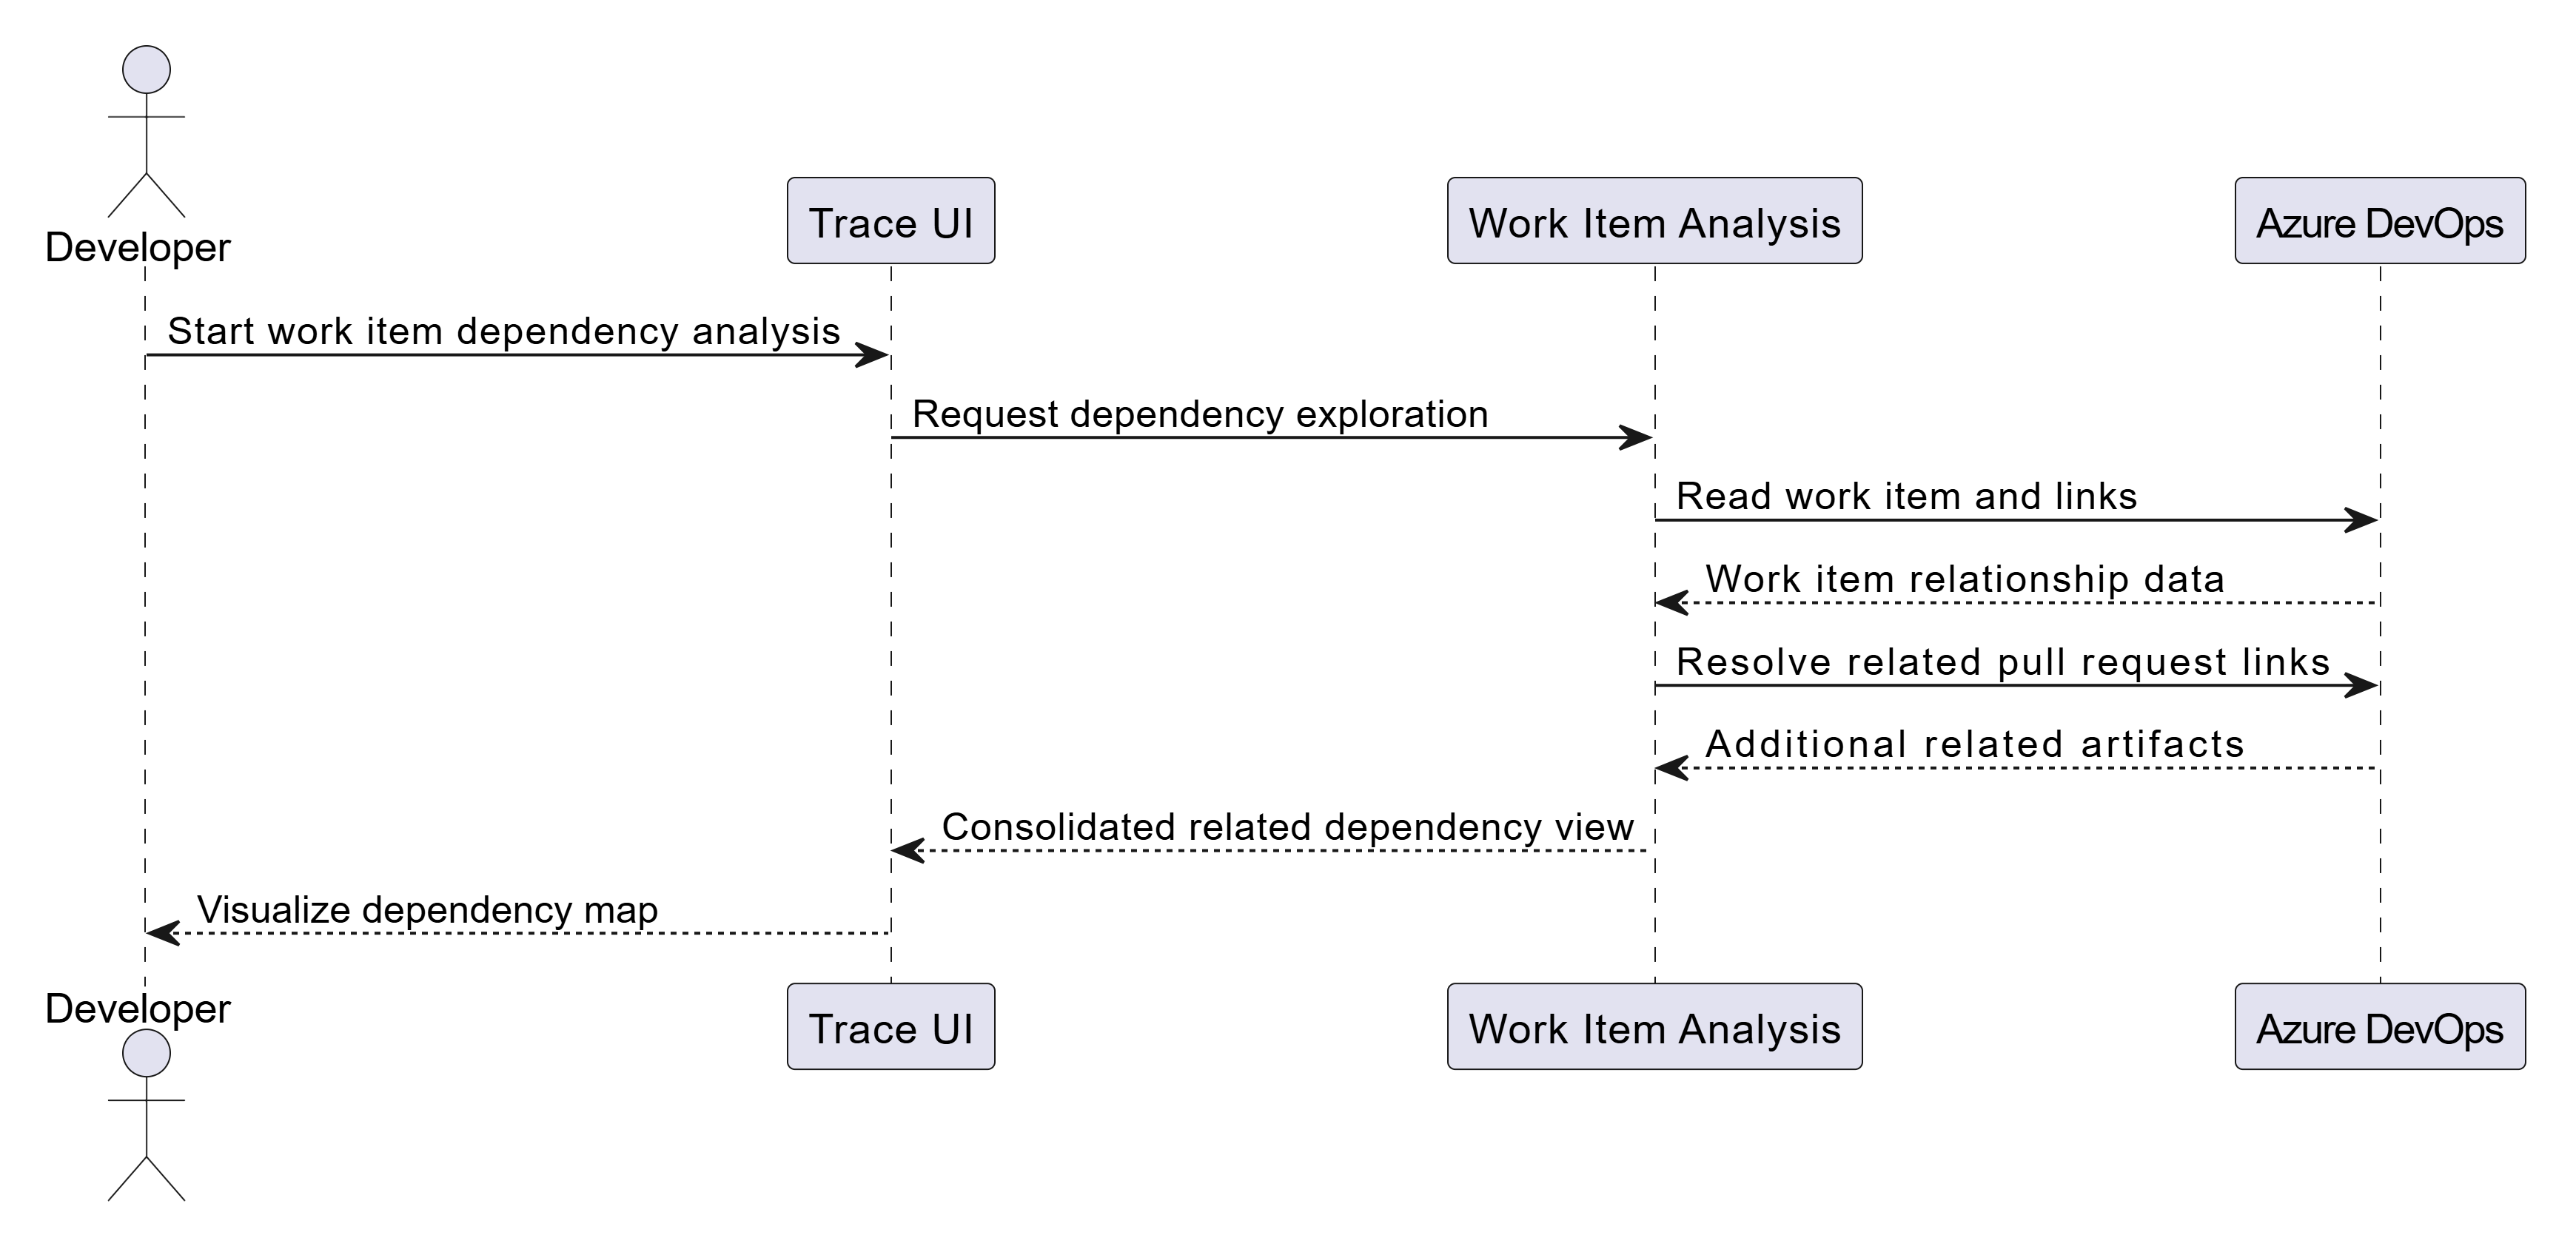
\includegraphics[width=\linewidth]{img/archi/workitemsequence.png}
  \caption{Sequence diagram — Work Item Management Component.}
  \label{fig:workitem-sequence}
\end{figure}

% ─────────────────────────────────────────────────────────────────────────────
\subsection{Pull Request Resolution Component}
\label{subsec:pr-component}

\subsubsection{Role and Responsibility}

The Pull Request Resolution Component bridges the work tracking domain and the
source control domain. Its function is to receive the pull request identifiers
extracted by the Work Item Management Component and resolve them into enriched,
normalized structures that carry both pull request metadata and the identities
of the repositories involved.

This bridging role is architecturally significant. In Azure DevOps, the
connection between a work item and the code changes that implement it passes
through pull requests: a work item links to a pull request, which links to one
or more commits in a specific repository. Without explicit pull request
resolution, the traceability chain would break at the boundary between the work
tracking system and the Git system.

\subsubsection{Pull Request Enrichment Process}

For each pull request identifier received, the component performs the following
operations:

\begin{enumerate}
  \item Query the Azure DevOps Git API for the full pull request metadata,
  including title, status, source branch, target branch, and the identifier of
  the repository in which the PR was created.
  \item Extract the list of work items formally linked to the pull request on
  the Git side — which may differ from the work items that link to the PR on
  the work tracking side.
  \item Construct a normalized \texttt{PullRequestSummaryDto} that exposes the
  PR identifier, the repository name, and the list of associated work item
  references in a stable, contract-conformant form.
\end{enumerate}

\subsubsection{Relationship to Other Components}

The Pull Request Resolution Component serves two consumer roles within the
pipeline. First, it directly enriches the dependency graph produced by the
Work Item Management Component by adding repository-level context to the PR
references identified during traversal. Second, it acts as a prerequisite for
the Commit Aggregation Component: resolving commits requires knowing which
repositories are involved, and this information is produced by pull request
resolution.

\subsubsection{Exposed API Surface}

\begin{itemize}
  \item \texttt{GET /pullrequests/:prId/workitems} — Resolves a pull request
  by its identifier and returns the normalized PR summary together with the
  work items formally linked to it on the Git side.
\end{itemize}

\begin{figure}[htbp]
  \centering
  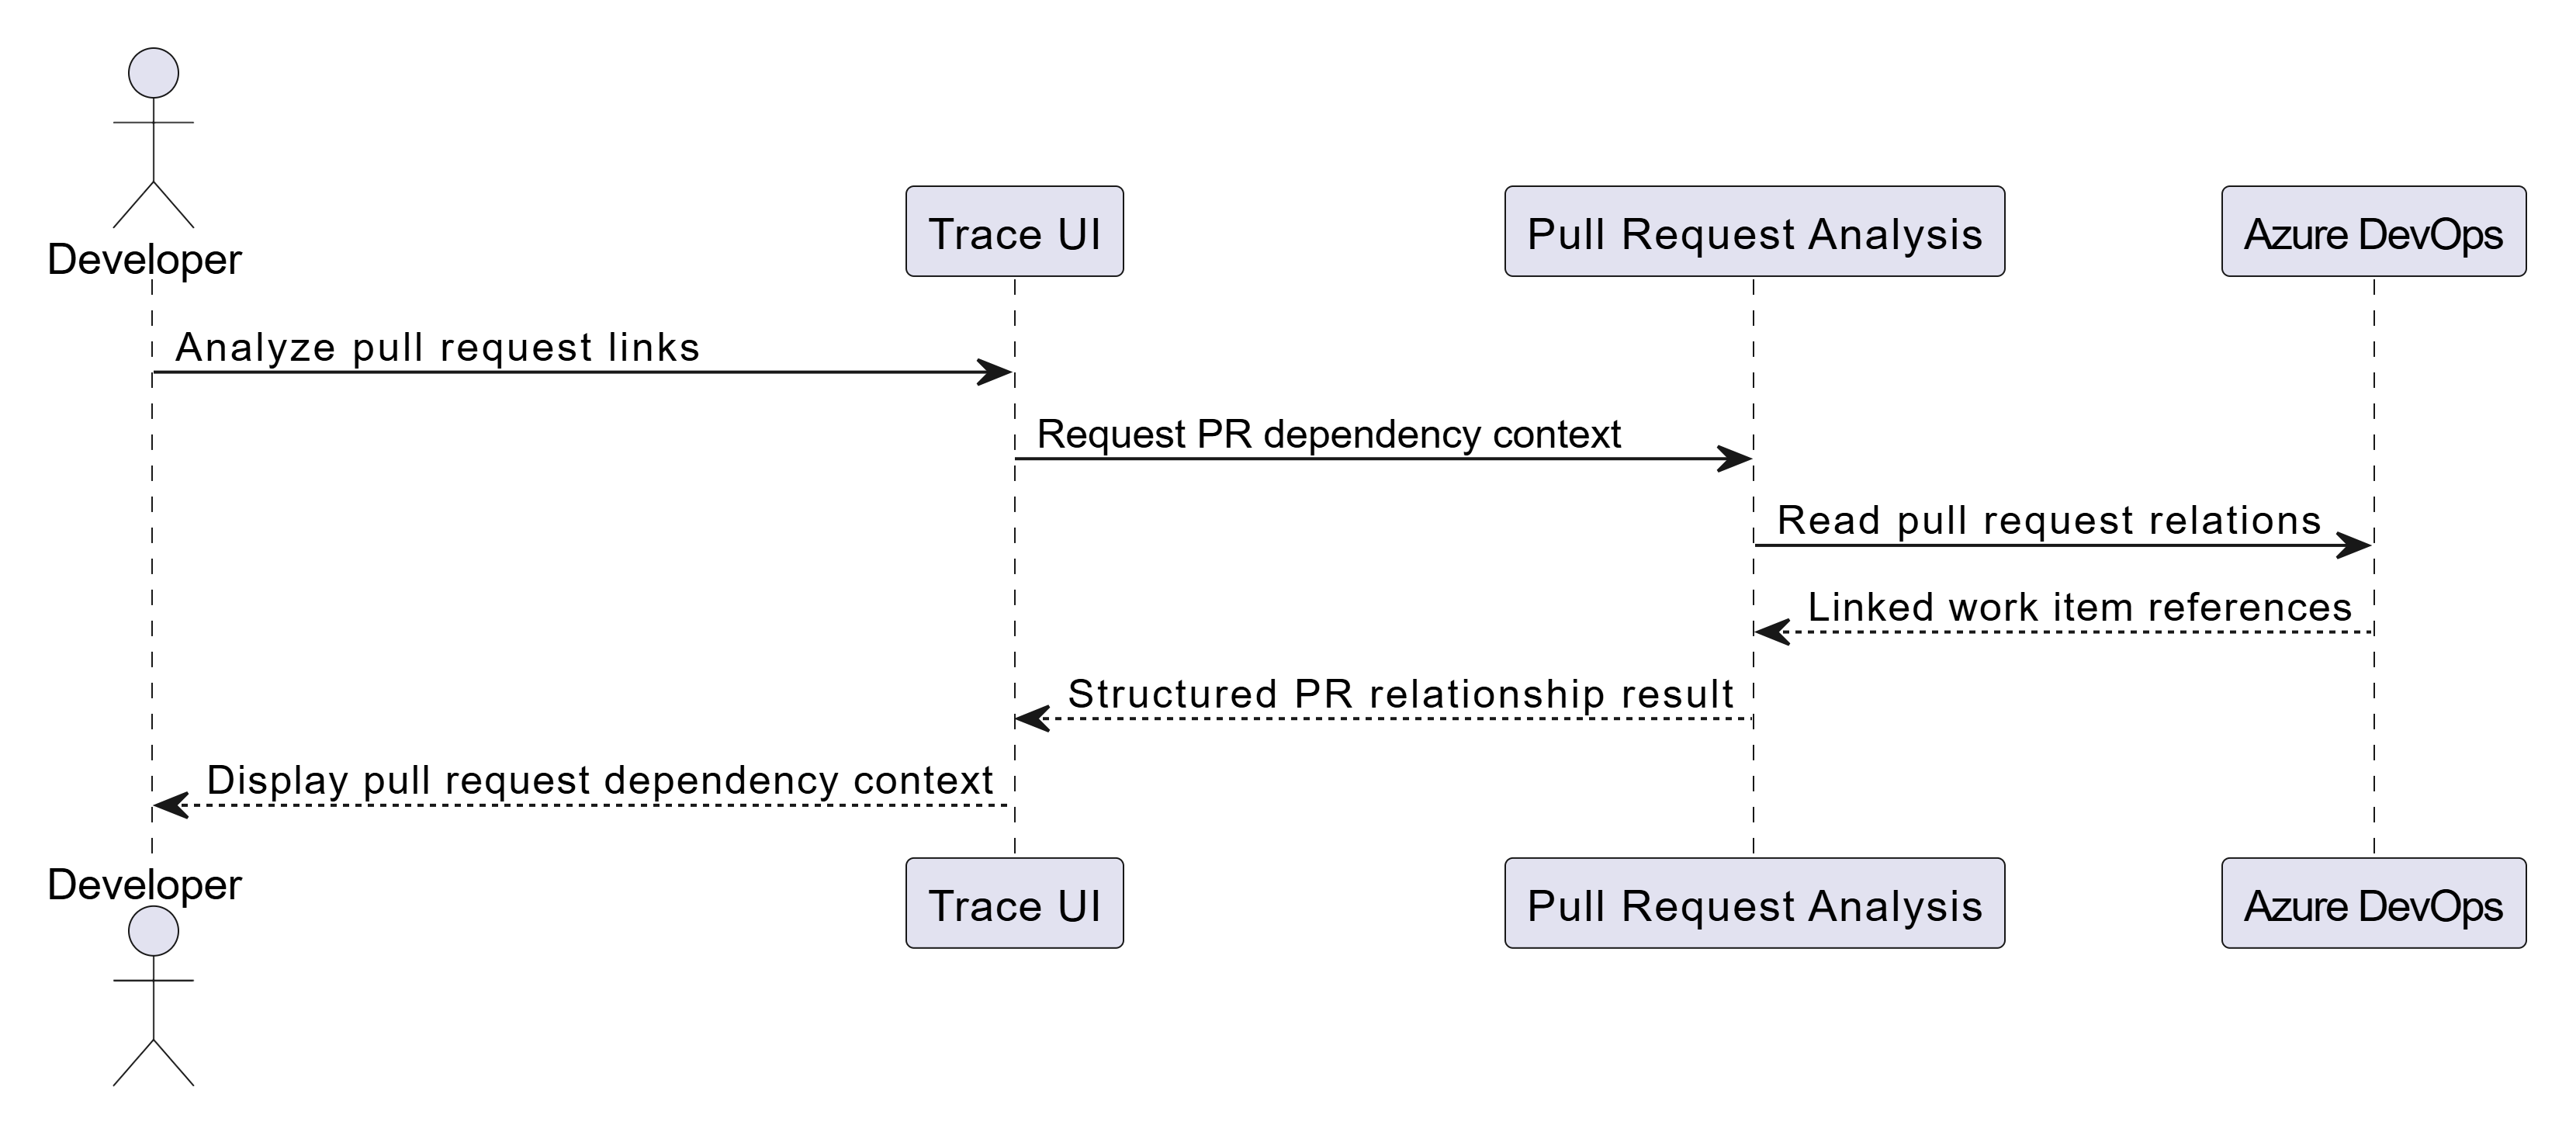
\includegraphics[width=\linewidth]{img/archi/pullrequest.png}
  \caption{Sequence diagram — Pull Request Resolution Component.}
  \label{fig:pullrequest-sequence}
\end{figure}

% ─────────────────────────────────────────────────────────────────────────────
\subsection{Commit Aggregation Component}
\label{subsec:commit-component}

\subsubsection{Role and Responsibility}

The Commit Aggregation Component delivers the finest level of traceability in
the system: it connects work items and pull requests to the actual code changes
that implement them, and it enriches those code changes with the repository
context — branches and tags — needed to determine their position relative to
software releases.

This component answers a critical question that no other layer of the system
addresses: for a given work item or pull request, which commits exist in which
repositories, and what is their release context?

\subsubsection{Commit Resolution Strategy}

The component resolves commits through two complementary mechanisms:

\begin{itemize}
  \item \textbf{Commit resolution via pull request}: The Azure DevOps Git API
  provides the list of commits that were merged as part of a specific pull
  request. This is the primary and most reliable mechanism for establishing
  the work-item-to-commit link when a pull request is present.
  \item \textbf{Commit resolution via work item}: For work items that carry
  direct commit references in their relation metadata, the component resolves
  those references directly through the Work Item Tracking API. This mechanism
  handles scenarios where commits are linked without a formal pull request.
\end{itemize}

In both cases, the resolved commits are deduplicated by commit identifier before
being passed downstream, ensuring that commits referenced through multiple paths
— which is common in complex branching strategies — appear only once in the
result.

\subsubsection{Repository Context Enrichment}

Resolving the commit list is not sufficient for release analysis. Each commit
must also be placed in its repository context: which branches contain it, and
which tags are associated with it. This context is critical for the Decision
Aggregation Component to determine whether a commit falls before or after a
specific release tag.

The component retrieves this context through the Azure DevOps Git API, querying
branch and tag references for each resolved commit. To avoid the prohibitive
cost of issuing one API call per commit, the component applies the
batch-oriented processing principle: it groups commit identifiers by repository
and resolves tag context in a single batched request per repository group.

The tag resolution strategy uses a \emph{latest-tag branch strategy}: for each
commit, the component identifies the most recent tag reachable from the commit
on the relevant branch, providing a meaningful release reference even when a
commit is not directly tagged.

\subsubsection{Internal Service Decomposition}

To maintain clarity and testability, the commit resolution logic is distributed
across four specialized internal services rather than concentrated in a single
large service class:

\begin{itemize}
  \item \textbf{CommitPRService}: resolves commits associated with a specific
  pull request via the Git API.
  \item \textbf{CommitWorkItemService}: resolves commits directly linked to a
  specific work item via the Work Item Tracking API.
  \item \textbf{CommitHistoryService}: queries commit history, branch
  references, and tag references for specific commits and repositories.
  \item \textbf{Utility services}: provide tag selection logic, batch reference
  resolution, and commit deduplication shared across the other services.
\end{itemize}

\subsubsection{Exposed API Surface}

\begin{itemize}
  \item \texttt{GET /commits/workitems/:workItemId} — Returns the deduplicated
  list of commits linked to the specified work item, resolved through both
  direct links and PR expansion.
  \item \texttt{GET /commits/pullrequests/:prId} — Returns the commits
  associated with the specified pull request.
  \item \texttt{GET /commits/branches} — Lists branch and tag names for a
  specified repository.
  \item \texttt{GET /commits/tags} — Resolves branch and tag references
  associated with a specific commit hash.
  \item \texttt{GET /commits/tags/batch} — Batch-resolves tag context for
  multiple commits across one or more repositories in a single request.
\end{itemize}

\begin{figure}[htbp]
  \centering
  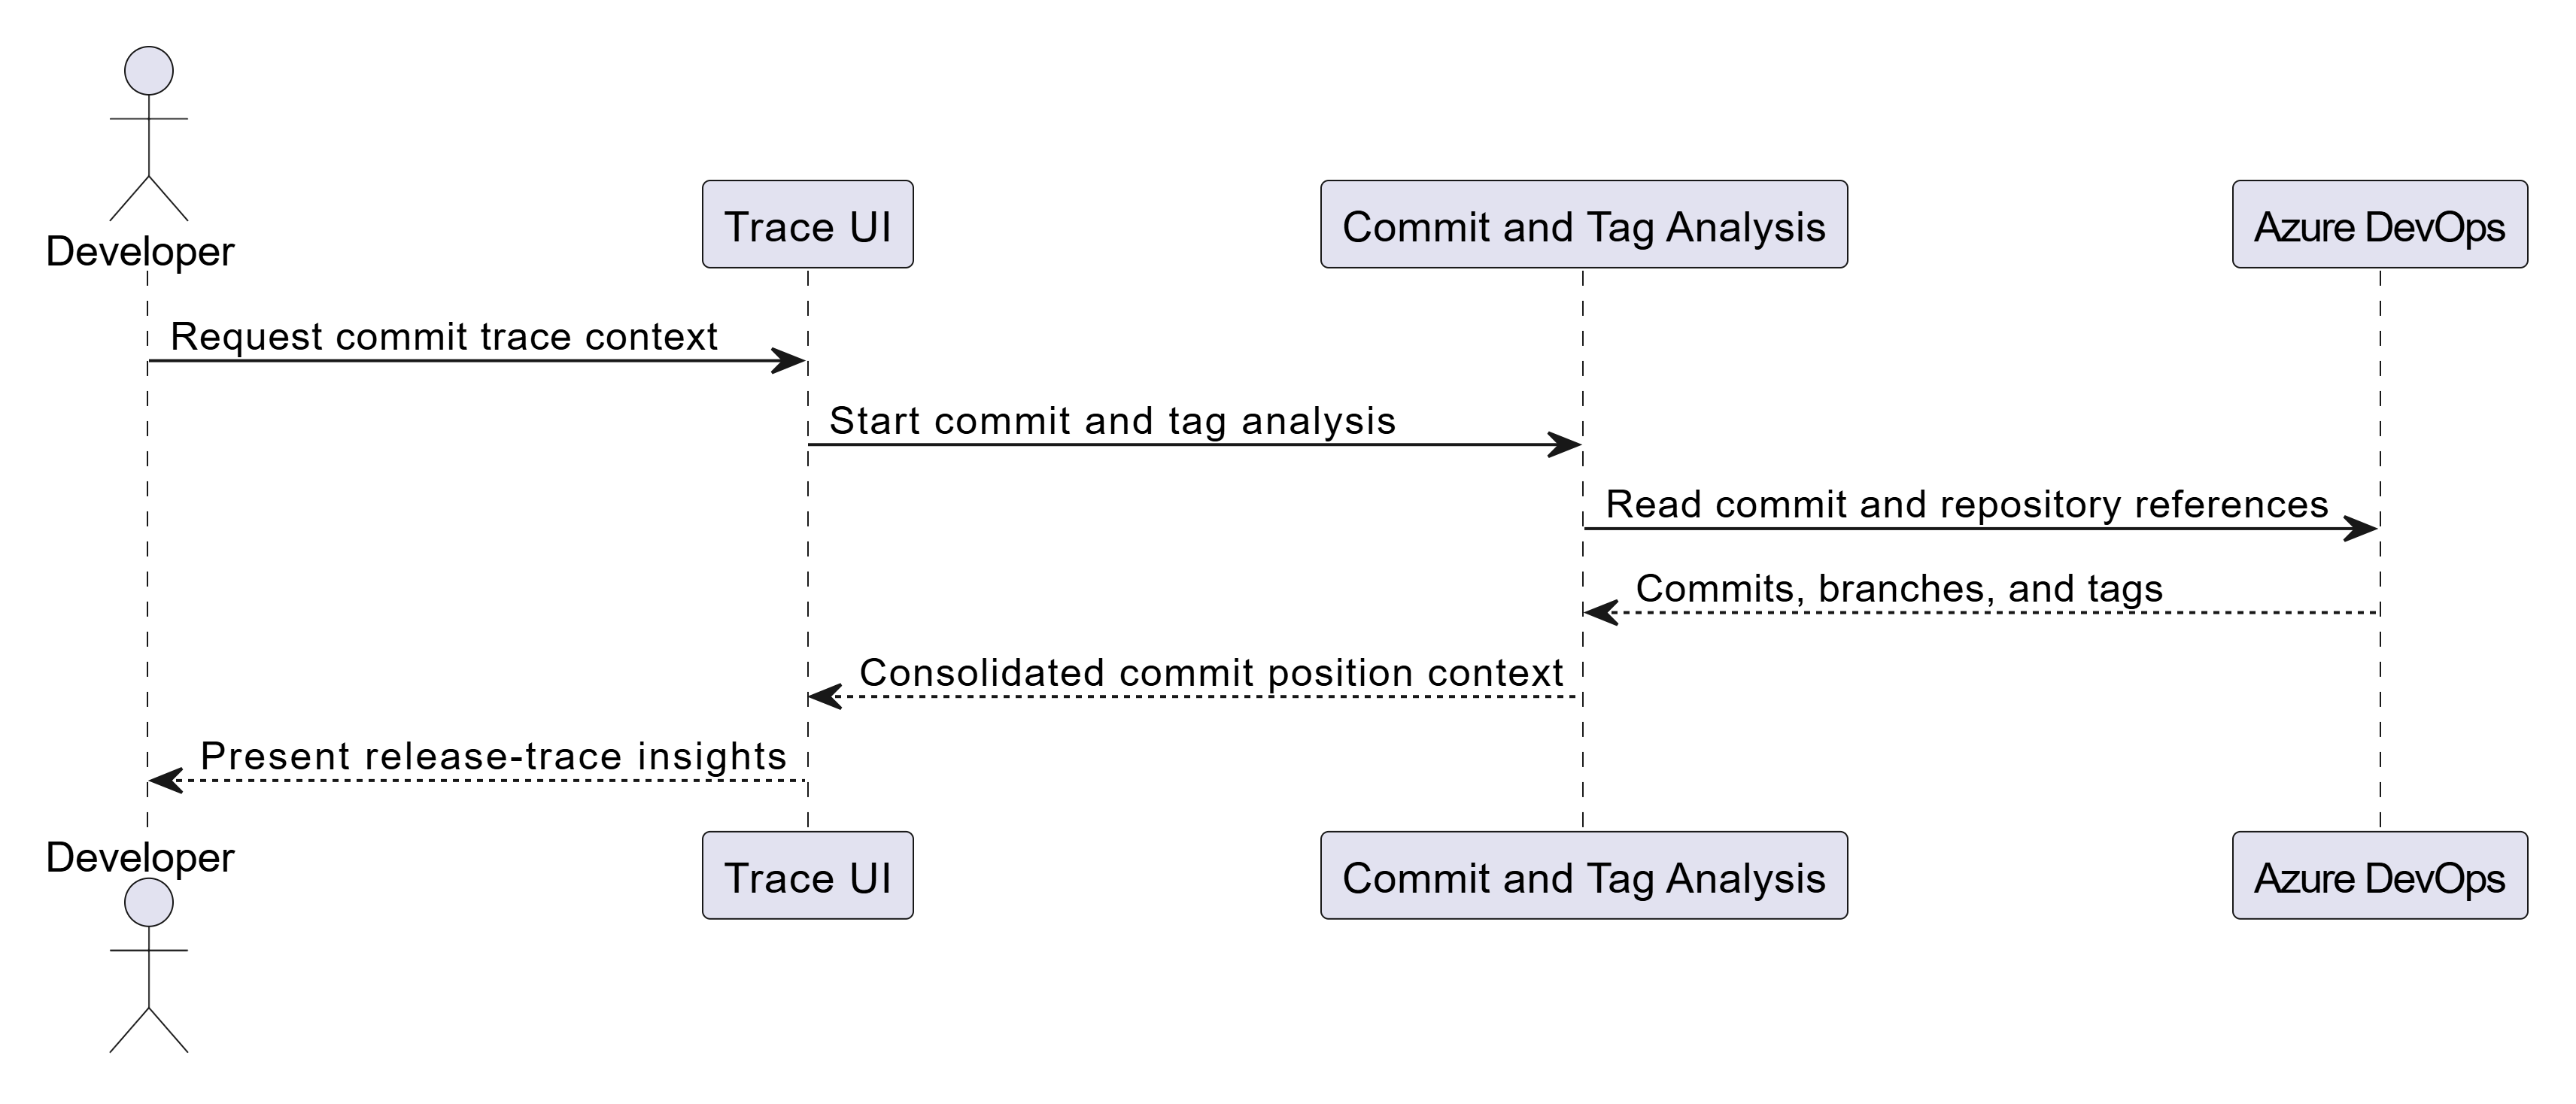
\includegraphics[width=\linewidth]{img/archi/commit.png}
  \caption{Sequence diagram — Commit Aggregation Component.}
  \label{fig:commit-sequence}
\end{figure}

% ─────────────────────────────────────────────────────────────────────────────
\subsection{Decision Aggregation Component}
\label{subsec:decision-component}

\subsubsection{Role and Responsibility}

The Decision Aggregation Component represents the final analytical stage of the
traceability pipeline. Unlike the three preceding components, it does not issue
any queries to Azure DevOps. Instead, it operates entirely on the normalized
data produced and collected by the upstream components, applying a classification
logic that transforms raw trace data into a structured, decision-ready output.

The central question this component addresses is: \emph{given the full set of
work items and their associated commits, what is the release readiness status
of each repository involved in the dependency graph?}

\subsubsection{Classification Logic}

The component receives a consolidated trace payload — containing work items with
their states, pull request summaries, and per-repository commit lists with tag
context — and applies a multi-step classification process:

\begin{enumerate}
  \item \textbf{Work item status partitioning}: work items are divided into two
  groups based on their current Azure DevOps state — those whose state maps to
  a \emph{done} condition (e.g., Closed, Resolved, Done) and those whose state
  indicates remaining work (e.g., Active, In Progress, New). This partition
  establishes whether the functional requirements carried by the work items have
  been fully delivered.

  \item \textbf{Repository commit classification}: for each repository present
  in the commit trace, the component examines the tag context of the associated
  commits and classifies the repository into one of three release-relative
  buckets:
  \begin{itemize}
    \item \textbf{Before-and-after}: the repository contains commits both before
    and after the reference tag, indicating that changes straddle a release
    boundary.
    \item \textbf{Only-before}: all commits in the repository predate the
    reference tag, indicating that the changes were fully included in the
    referenced release.
    \item \textbf{Only-after}: all commits in the repository postdate the
    reference tag, indicating that the changes are part of a future release
    scope.
  \end{itemize}

  \item \textbf{Pull request relevance marking}: when a commit should be
  highlighted for pull request integration, the component sets a dedicated
  \texttt{considerForPR} flag in the output. This makes the recommendation
  explicit without forcing the user to infer it from raw tag data.
\end{enumerate}

\subsubsection{Stateless and Deterministic Design}

A key design property of this component is that it is entirely stateless and
deterministic. Given the same input trace payload, it will always produce the
same classification output. This property makes the component straightforward
to test, easy to reason about, and safe to invoke multiple times without side
effects.

The stateless design also means that the component can be invoked independently
of the rest of the pipeline — for example, to recompute a decision view when
the user changes the reference tag — without needing to repeat the upstream
data collection steps.

\subsubsection{Exposed API Surface}

\begin{itemize}
  \item \texttt{POST /decision/aggregate} — Accepts a structured trace payload
  and returns the classified decision output, including the work item status
  partition, per-repository decision buckets, and commit-level PR relevance
  flags.
\end{itemize}

\begin{figure}[htbp]
  \centering
  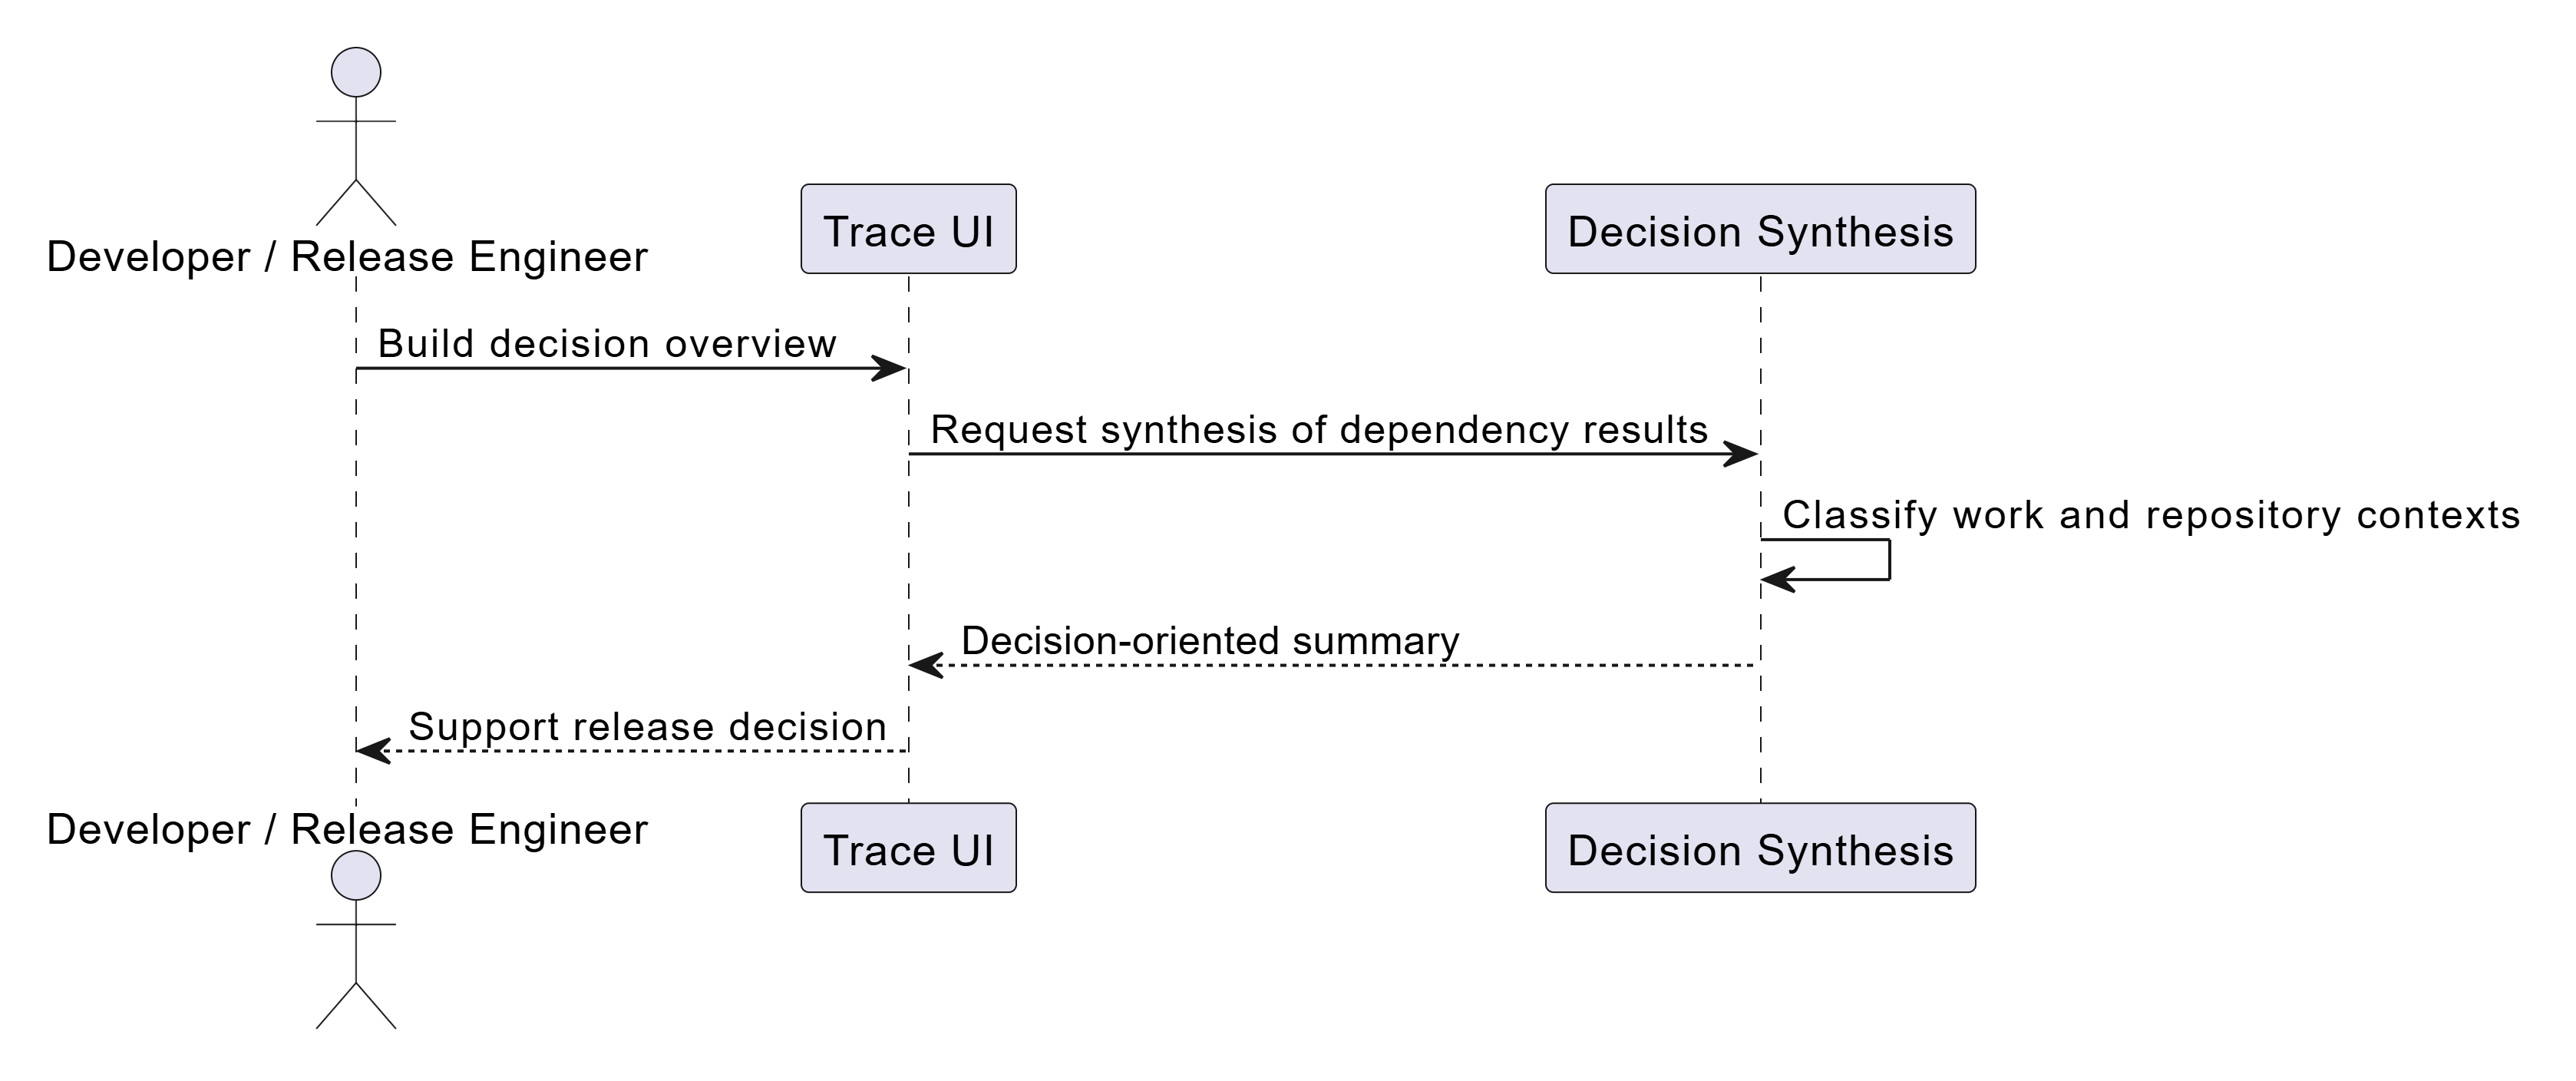
\includegraphics[width=\linewidth]{img/archi/decision.png}
  \caption{Sequence diagram — Decision Aggregation Component.}
  \label{fig:decision-sequence}
\end{figure}


% ─────────────────────────────────────────────────────────────────────────────
\section{Data Contracts and Normalization Model}
\label{sec:data-contracts}

A critical structural element of the proposed solution is its systematic use of
Data Transfer Objects (DTOs) as the exclusive mechanism for data exchange across
module boundaries, API surfaces, and layer transitions. This section describes
the data contract model and the normalization strategy that underlies it.

\subsection{Role of Data Transfer Objects}

DTOs serve two distinct but complementary roles in the system. At the
\textbf{input} boundary, they enforce the structure and validity of data
entering a module — whether from the Presentation Layer or from an upstream
pipeline stage. At the \textbf{output} boundary, they define the stable,
documented shape of data that a module guarantees to its consumers.

This dual role means that every data transformation in the system is explicit
and traceable. When a developer reads the output DTO of a module, they have a
complete and accurate description of what that module produces — not an implicit
understanding derived from reading implementation code.

\subsection{Main Data Contract Groups}

The system defines five primary groups of data contracts:

\begin{itemize}
  \item \textbf{Work Item Contracts}: \texttt{WorkItemDto} represents one
  normalized work item with its identifier, title, type, state, assignee, and
  typed relation links through \texttt{WorkItemLinkDto}. Single-root traversal
  results are wrapped in \texttt{RelatedWorkItemsDataDto}, while multi-root
  traversals use \texttt{RelatedWorkItemsBatchDataDto}.

  \item \textbf{Pull Request Contracts}: \texttt{PullRequestSummaryDto}
  provides a lightweight normalized representation of a pull request within the
  traceability context, exposing the PR identifier and the repository name. This
  DTO is embedded in both work item trace responses and pull request module
  responses, creating a consistent cross-module reference.

  \item \textbf{Commit and Repository Contracts}: \texttt{CommitInfo} carries
  the commit identifier and repository name as a minimal reference embedded in
  trace responses. Richer DTOs — \texttt{CommitsByWorkItemResponseDto},
  \texttt{CommitsByPRResponseDto}, \texttt{RepoReferencesResponseDto} — provide
  full commit lists with branch and tag context for consuming components.

  \item \textbf{Streaming Event Contracts}: SSE messages carry structured
  payloads defined by dedicated event DTOs. Batch progress messages expose the
  batch content, the batch sequence number, and the cumulative count of resolved
  items. Completion and error messages follow distinct schemas to allow the
  consumer to unambiguously identify the event type.

  \item \textbf{Decision Contracts}: the input payload of the final
  classification stage is described by \texttt{DecisionAggregateInputDto}, and
  the output is described by \texttt{DecisionAggregateOutputDto}. Together,
  they define the work item status groups, repository-level decision buckets,
  and commit-level pull request relevance flags returned by the system.
\end{itemize}

\subsection{Normalization at the Integration Boundary}

All normalization from raw Azure DevOps API responses to internal DTOs occurs
at the Integration Layer boundary, within shared utility functions dedicated to
this transformation. These utilities handle the structural parsing of Azure
DevOps relation types, the extraction of embedded identifiers (such as pull
request IDs encoded in work item relation URLs), and the mapping of Azure
DevOps field names to the internal model.

This boundary normalization ensures that no module ever encounters raw Azure
DevOps response data in its processing logic. All processing, classification,
and enrichment operates on a clean, homogeneous internal model.


% ─────────────────────────────────────────────────────────────────────────────
\section{End-to-End Data Flow}
\label{sec:data-flow}

The four core components operate together in a clear, sequential pipeline that
connects user intent to actionable analytical output. This section traces the
complete execution path of an analysis session, illustrating how each component
contributes to the progressive enrichment of the dependency graph.

\begin{figure}[htbp]
  \centering
  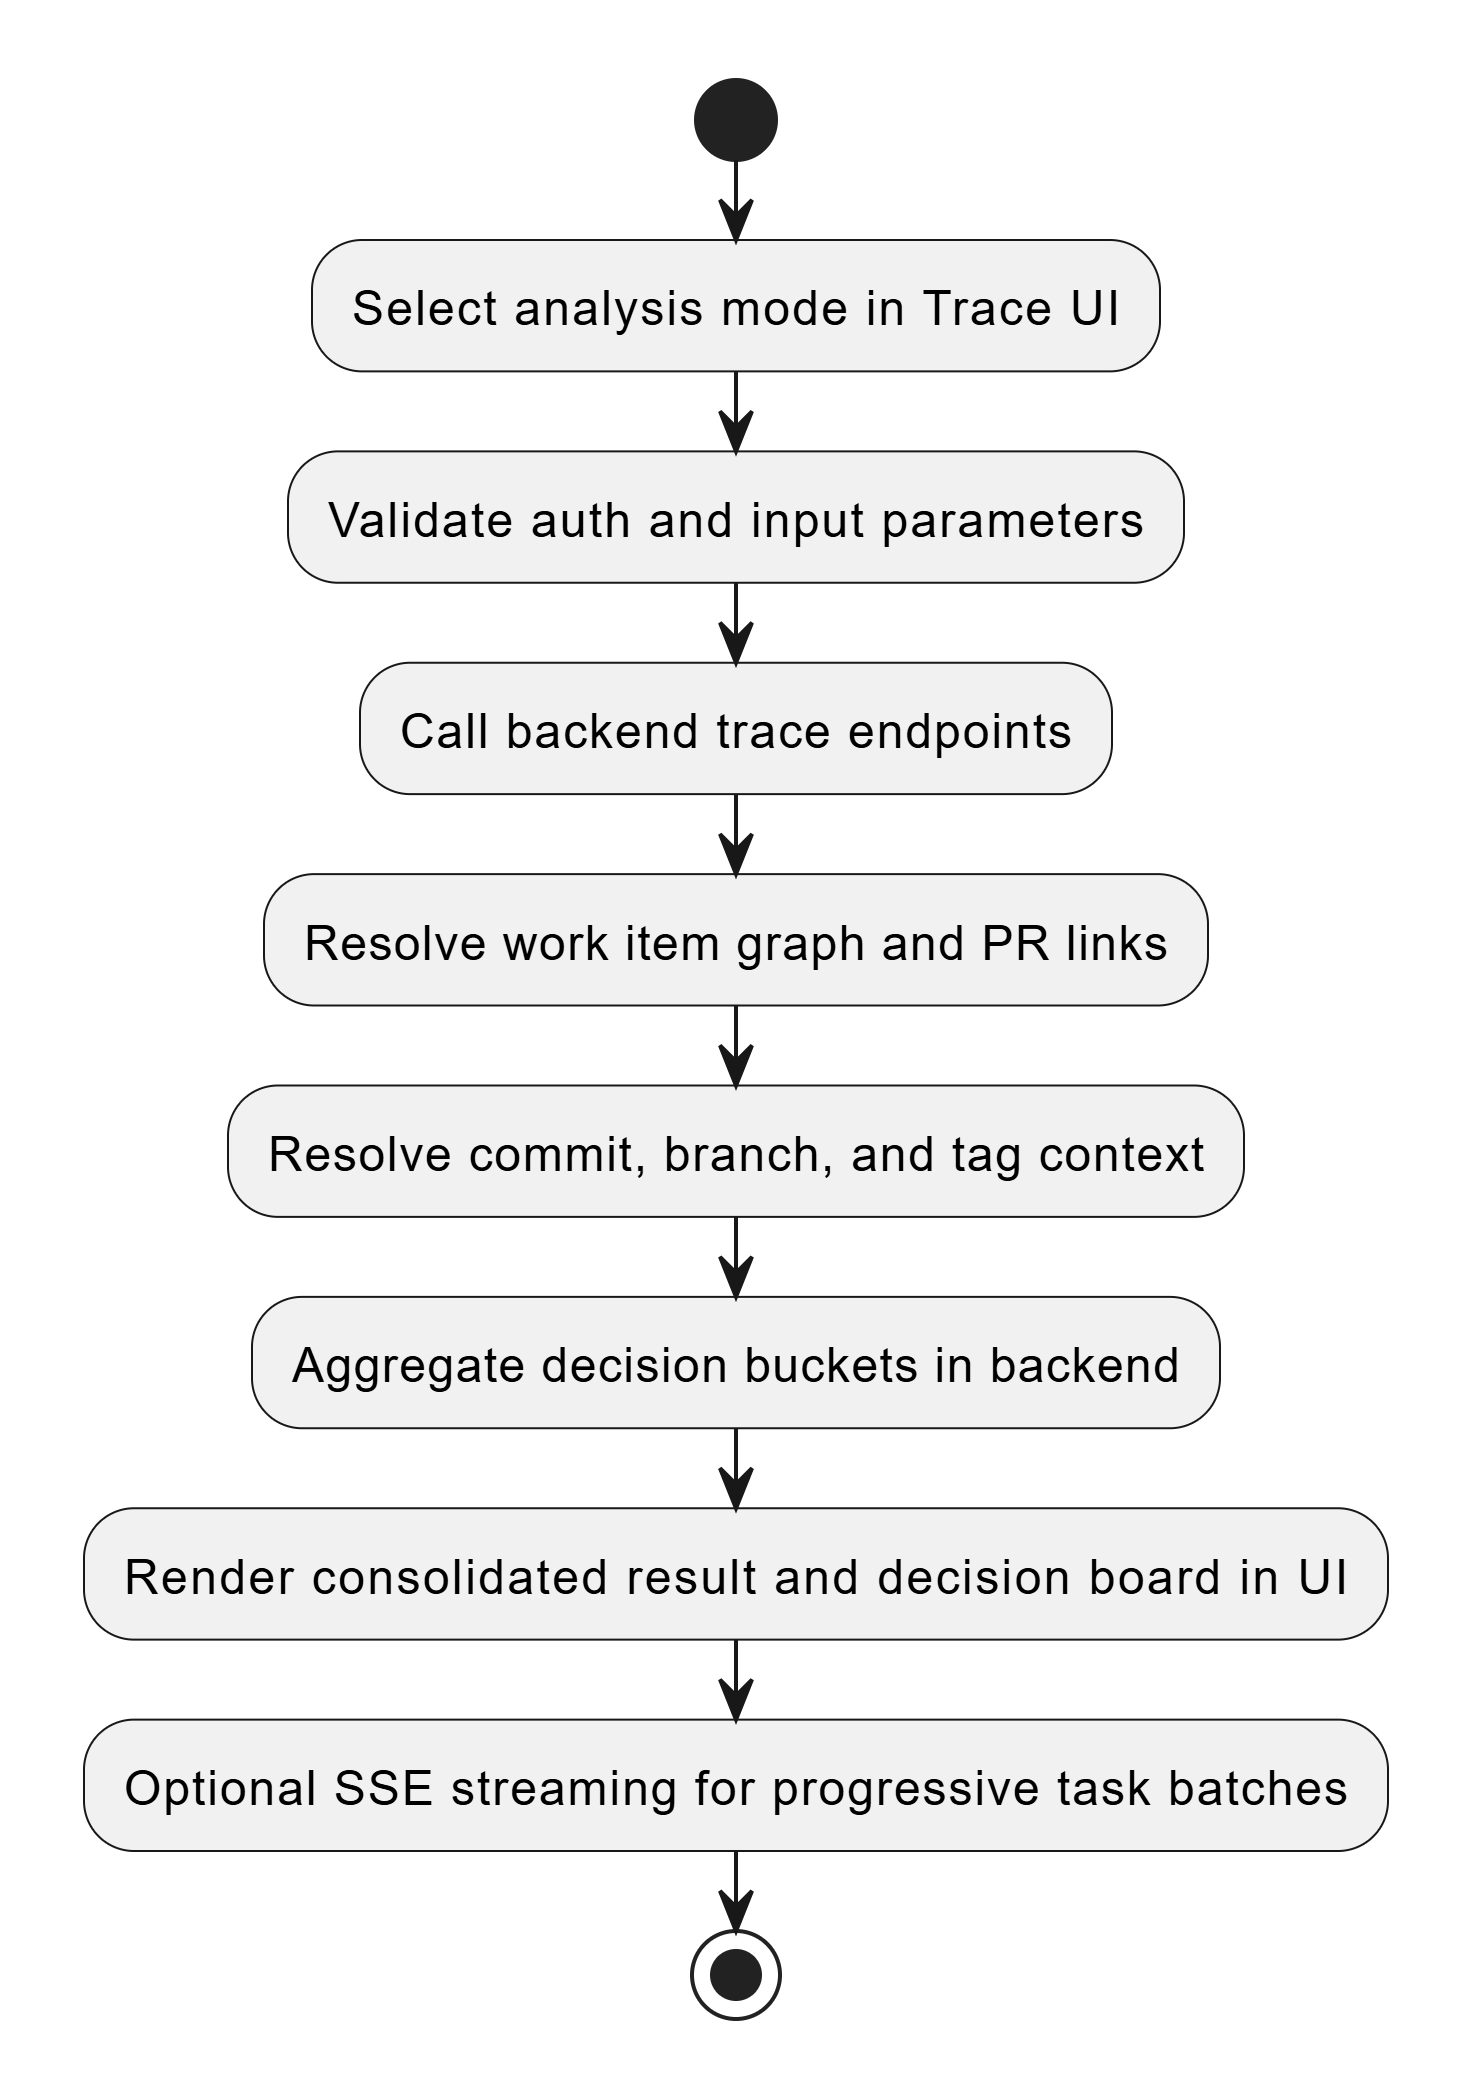
\includegraphics[width=\linewidth]{img/archi/end_end.png}
  \caption{End-to-end data flow across the four system components.}
  \label{fig:end-to-end-flow}
\end{figure}

\subsection{Step 1 — User Initiates the Analysis}

The user accesses the Trace UI and selects an analysis mode. In single-trace
mode, the user provides a single work item identifier. In batch mode, the user
selects multiple work items from a streamed task list. In batch-related mode,
the user triggers an aggregated analysis across all selected roots simultaneously.

The UI validates the user input and constructs a well-formed request that
includes the work item identifiers, the Azure DevOps project context, and any
additional parameters such as the analysis depth or the reference tag for
decision classification.

\subsection{Step 2 — Work Item Graph Construction}

The request reaches the backend, where the Work Item Management Component begins
the dependency graph traversal. It retrieves the specified root work items from
the Azure DevOps Work Item Tracking API and expands the graph level by level,
following parent/child and related-item links. Visited states are tracked to
prevent cycles. Items are retrieved in batches, and results are cached to avoid
redundant calls.

At the end of this stage, the component has produced:
\begin{itemize}
  \item a complete, normalized list of all work items reachable from the
  specified roots;
  \item a deduplicated list of pull request identifiers extracted from the
  relation metadata of visited work items.
\end{itemize}

\subsection{Step 3 — Pull Request Resolution and Repository Identification}

The Pull Request Resolution Component receives the list of pull request
identifiers produced in the previous stage. For each identifier, it queries the
Azure DevOps Git API to retrieve the PR metadata and the list of work items
formally linked to the PR on the Git side. It constructs a normalized
\texttt{PullRequestSummaryDto} for each PR, capturing the repository name
alongside the PR identifier.

At the end of this stage, the dependency graph has been enriched with:
\begin{itemize}
  \item normalized pull request summaries associated with the relevant work
  items;
  \item the repository identities of all repositories involved in the analysis.
\end{itemize}

\subsection{Step 4 — Commit Resolution and Repository Context Enrichment}

The Commit Aggregation Component uses the pull request summaries and repository
identifiers produced in the previous stage to resolve commits. For each pull
request, it queries the Git API to retrieve the list of commits merged as part
of that PR. For work items with direct commit links, it resolves those commits
independently.

All resolved commits are deduplicated and grouped by repository. The component
then performs batch tag resolution: for each repository group, it issues a
single API request to resolve the branch and tag context of all relevant commits
simultaneously.

At the end of this stage, the dependency graph is complete in the sense that
every artifact in the traceability chain — from work item to commit — is
represented, normalized, and enriched with release context.

\subsection{Step 5 — Decision Classification}

The Decision Aggregation Component receives the fully enriched trace payload
and applies its classification logic. Work items are partitioned by completion
state. Repositories are classified into release-relative decision buckets based
on the tag context of their associated commits. Commits of particular relevance
for pull request integration are flagged accordingly.

The output is a structured decision payload that directly answers the
release-readiness question: which repositories are fully integrated, which
straddle a release boundary, and which remain outside the current release scope.

\subsection{Step 6 — Result Delivery and Visualization}

The classified decision payload, together with the full trace data, is returned
to the Trace UI. The UI assembles the final view state and renders the results
across its specialized view components: the dependency graph view for work item
hierarchies, the repository grouping view for commit-level context, and the
Decision Dashboard for release classification output.

The user can interact with the results, drill down into specific work items or
repositories, and use the Decision Dashboard output to inform release, integration,
and escalation decisions.


% ─────────────────────────────────────────────────────────────────────────────
\section{User Interface Design and Interaction Model}
\label{sec:ui-design}

Although the backend performs the core analysis, the value of the system also
depends on how clearly the results are exposed to end users. This section
summarizes the three analysis modes supported by the Trace UI and explains the
type of user interaction expected in each case.

\subsection{Single Work Item Trace Mode}

In this mode, the user enters one work item identifier and launches a focused
analysis. The system traverses the dependency graph rooted at that item,
resolves the related pull requests and commits, and presents the result in a
structured view. This mode is well suited to targeted impact analysis, for
example when verifying the implementation scope of a specific user story.

\subsection{Batch Work Item Trace Mode}

In batch mode, the user receives a progressively loaded list of available work
items through the SSE endpoint, selects several of them, and then launches a
group analysis. This mode is useful when preparing a release or reviewing a
sprint scope, because it reveals all repositories and commits involved in the
selected set.

\subsection{Batch-Related Work Item Trace Mode}

This mode performs a parallel dependency analysis across all selected roots and
then consolidates the result. The work items can be ranked by the breadth of
their dependency footprint, and the Decision Dashboard is displayed to support
release-oriented interpretation of the aggregated result.

\subsection{Observability and Progress Feedback}

One important design objective of the Trace UI is to keep users informed during
long-running analyses. Thanks to streaming, results appear progressively instead
of after one long blocking delay. The interface also exposes the SSE connection
state --- connecting, open, reconnecting, or closed --- so that users can
understand what the system is doing at each stage of the analysis.


% ─────────────────────────────────────────────────────────────────────────────
\section{Operational Observability and Logging Strategy}
\label{sec:observability}

Operational observability is treated as a first-class system property, not an
afterthought. The system implements a structured logging strategy using the
\textbf{AppLogger} framework, applied consistently across all backend modules
and service layers.

\subsection{Log Level Strategy}

Different log levels are used strategically across the pipeline to maintain a
clean operational signal while preserving diagnostic depth when needed:

\begin{itemize}
  \item \texttt{log}: normal operation events — component invocations,
  traversal progress, batch boundaries, and successful API call completions.
  These form the standard operational trace of a healthy analysis session.
  \item \texttt{warn}: recoverable anomalies — partial data returns, unexpected
  API response shapes, rate limit proximity signals, and items skipped due to
  missing relations. These do not interrupt processing but indicate conditions
  worth monitoring.
  \item \texttt{error}: failures requiring attention — API call failures after
  retry exhaustion, data normalization failures, and unresolvable dependency
  links. These are logged with full context to support root cause analysis.
  \item \texttt{debug} and \texttt{verbose}: detailed diagnostic output —
  individual work item relation resolution, cache hit/miss events, batch
  composition details, and tag resolution results. These are intended for
  development and troubleshooting and are suppressed in normal operation.
\end{itemize}

\subsection{Observability Value in a Traceability System}

Structured logging is especially valuable in a system that depends on external
APIs for correctness. When an analysis produces unexpected results — a missing
commit, an incomplete graph, or an incorrect decision classification — structured
logs allow the developer or operator to reconstruct the exact sequence of API
calls and data transformations that led to the output, without requiring a
debugger or a reproduction environment.

The logging strategy also provides an audit trail for analysis sessions, which
can be used to verify that a specific analysis was performed correctly and to
compare results across successive sessions.


% ─────────────────────────────────────────────────────────────────────────────
\section{System Advantages}
\label{sec:advantages}

The proposed solution delivers concrete advantages over the current state of
practice, addressing both the functional gaps identified in the problem analysis
and broader non-functional requirements of reliability, scalability, and
maintainability.

\subsection{Centralized and Unified Visibility}

The most immediate advantage of the solution is the consolidation of scattered
dependency information into a single, coherent analytical interface. Before this
system, understanding the full dependency chain of a work item required a
developer or release engineer to navigate across multiple Azure DevOps views —
the work item board, the pull request list, the repository commit history, and
the branch/tag management interface — and manually correlate the information
found in each.

The proposed system eliminates this manual correlation step. A single analysis
session retrieves, normalizes, enriches, and presents the complete dependency
chain from work item to commit, in a structured format that supports immediate
decision-making.

\subsection{Improved Release Decision Support}

The Decision Aggregation Component translates raw trace data into a structured
release classification that directly answers the questions relevant to a release
decision: which repositories are fully integrated, which straddle the release
boundary, and which changes fall outside the current scope. This structured
output reduces the time required to assess release readiness and reduces the
risk of releasing incomplete or incorrectly integrated changes.

\subsection{Scalability for Large Projects}

The batch-oriented processing strategy, combined with in-memory caching and
SSE-based progressive delivery, makes the system viable for large projects with
deep dependency graphs. Analysis sessions involving dozens of root work items,
hundreds of related items, and thousands of commits across multiple repositories
can be completed efficiently and presented to the user with real-time progress
feedback — a use case that is practically infeasible with manual Azure DevOps
navigation.

\subsection{Consistency and Reliability of Results}

The systematic normalization of all Azure DevOps API responses at the integration
boundary ensures that analysis results are consistent and reliable regardless of
the structural variations present in the underlying data. Users can trust that
the same query will produce the same result across successive sessions, and that
changes in Azure DevOps API response structure will be absorbed at the
normalization layer without affecting the rest of the pipeline.

\subsection{Extensibility for Future Artifact Types}

The modular architecture of the Application Layer makes it straightforward to
extend the traceability scope beyond the artifact types supported in the current
version. New dependency types — such as pipeline run artifacts, automated test
results, release deployment records, or cross-project work item links — can be
introduced as new modules alongside the existing four, following the same
controller/service/DTO pattern and integrating into the pipeline through
well-defined data contracts. No modification to the existing modules or the core
traversal logic is required.

\subsection{Shared Reference for Cross-Functional Collaboration}

By providing a single, factual, and reproducible view of dependencies, the
system creates a shared reference that can be used consistently across roles.
Developers, release engineers, technical leads, and project managers can all
consult the same analysis output to discuss scope, impact, and readiness —
reducing misalignments that arise from each stakeholder navigating the same data
through different interfaces and arriving at different conclusions.


% ─────────────────────────────────────────────────────────────────────────────
\section{Conclusion}
\label{sec:solution-conclusion}

This chapter has presented the proposed solution for structured dependency
traceability in Azure DevOps environments. The system is designed around a
three-layer architecture, four fundamental design principles, and a sequential
pipeline of four specialized components that together transform user-provided
work item identifiers into a fully classified, decision-ready dependency view.

Several design decisions stand out as particularly significant. The adoption of
a contract-first, DTO-based data model ensures stability and consistency across
all module boundaries. The batch-oriented processing strategy makes the system
viable at scale without overwhelming external APIs. The integration of SSE-based
progressive streaming provides a responsive user experience even during
long-running analysis sessions. And the stateless, deterministic design of the
Decision Aggregation Component makes the classification logic transparent and
easily testable.

Together, these decisions produce a system that is not only functional today but
structured for extension and evolution as the traceability requirements of the
organization grow.

The following chapter details the technical implementation of this architecture:
the technologies, frameworks, and implementation patterns used to realize each
component, and the engineering decisions taken during the development process.